\documentclass[11pt,a4paper]{article}
\usepackage[a4paper,margin=2.3cm]{geometry}
\usepackage{fontspec}
\setmainfont{Noto Serif CJK TC}[BoldFont={Noto Serif CJK TC Bold}]
\setsansfont{Noto Sans CJK TC}[BoldFont={Noto Sans CJK TC Bold}]
\XeTeXlinebreaklocale "zh"
\XeTeXlinebreakskip = 0pt plus 1pt
\usepackage{amsmath,amssymb}
\usepackage{tabularx,booktabs,array}
\usepackage{enumitem}
\usepackage[most]{tcolorbox}
\usepackage{xcolor,graphicx}
\usepackage{hyperref}
\hypersetup{colorlinks=true,linkcolor=blue!50!black}
\setlength{\parindent}{0pt}
\setlength{\parskip}{0.5em}
\renewcommand{\arraystretch}{1.3}

\definecolor{bluebg}{HTML}{F5F8FB}  \definecolor{blueframe}{HTML}{AFC0D2}  \definecolor{bluetitle}{HTML}{1F3864}
\definecolor{greenbg}{HTML}{F3F9F4} \definecolor{greenframe}{HTML}{A8CDB1} \definecolor{greentitle}{HTML}{1E5631}
\definecolor{amberbg}{HTML}{FCF8EE} \definecolor{amberframe}{HTML}{DCC896} \definecolor{ambertitle}{HTML}{7A5200}
\newcommand{\boxmark}{\rule[0.02em]{0.62em}{0.62em}}
\tcbset{
  boxblue/.style ={colback=bluebg, colbacktitle=bluebg, colframe=blueframe, coltitle=bluetitle},
  boxgreen/.style={colback=greenbg,colbacktitle=greenbg,colframe=greenframe,coltitle=greentitle},
  boxamber/.style={colback=amberbg,colbacktitle=amberbg,colframe=amberframe,coltitle=ambertitle},
  notebox/.style={enhanced,breakable,sharp corners,boxrule=0.6pt,titlerule=0pt,
    fonttitle=\bfseries\large,toptitle=6pt,bottomtitle=2pt,
    left=10pt,right=10pt,top=4pt,bottom=8pt,before skip=10pt,after skip=12pt,boxblue}}
\newtcolorbox{takeaway}[1][重點提示]{notebox,boxamber,title={\boxmark\enspace #1}}
\newtcolorbox{derivationbox}[1][完整推導]{notebox,boxblue,title={\boxmark\enspace #1}}
\newtcolorbox{recipebox}[1][結論]{notebox,boxgreen,title={\boxmark\enspace #1}}

\begin{document}
\begin{center}
{\LARGE\bfseries\sffamily 課程學習回授：例 5.10 的根軌跡何時會變成「）（」形？}\\[0.4em]
{\large 控制系統 Unit 5 根軌跡 Root Locus\quad·\quad 2026/11/9}
\end{center}

\begin{takeaway}[摘要]
講義例 5.10 的迴路轉移函數 $L(s)=\dfrac{1}{s(s+2)[(s+1)^2+4]}$ 有複數重根。教授上課時提出有沒有可能畫成「）（」形。本報告說明：
\begin{enumerate}
  \item 若把複數極點改成 $-1\pm j\omega$ 且 $\omega<1$，根軌跡就會變成「）（」形；$\omega=1$ 是兩種形狀的分界。
  \item 五條規則中 Rule 1--4 的結果與 $\omega$ 完全無關，只有重根位置（Rule 5）會改變，所以只靠前四條規則無法決定形狀。
\end{enumerate}
\end{takeaway}

\textbf{說明}：第 2 節以後的推導與分類是我自己延伸的分析；所有數值與圖形都以 Python（\texttt{numpy.roots} 逐點掃描 $K$）驗算。

%==========================================
\section{問題來源}
講義例 5.10 的根軌跡是：實軸上 $0$、$-2$ 出發的分支在 $-1$ 會合後垂直分開，與複數極點 $-1\pm2j$ 往下／往上的分支在 $-1\pm1.22j$ 相遇（複數重根），再轉向漸近線。教授上課時提出：複數極點之間直接連一條垂直線，實軸分支往內走，另外兩條曲線呈「）（」形往漸近線延伸（圖 1）。問題是：\textbf{這種形狀有可能出現嗎？}本報告是我對這個課堂問題的回答。

\begin{center}
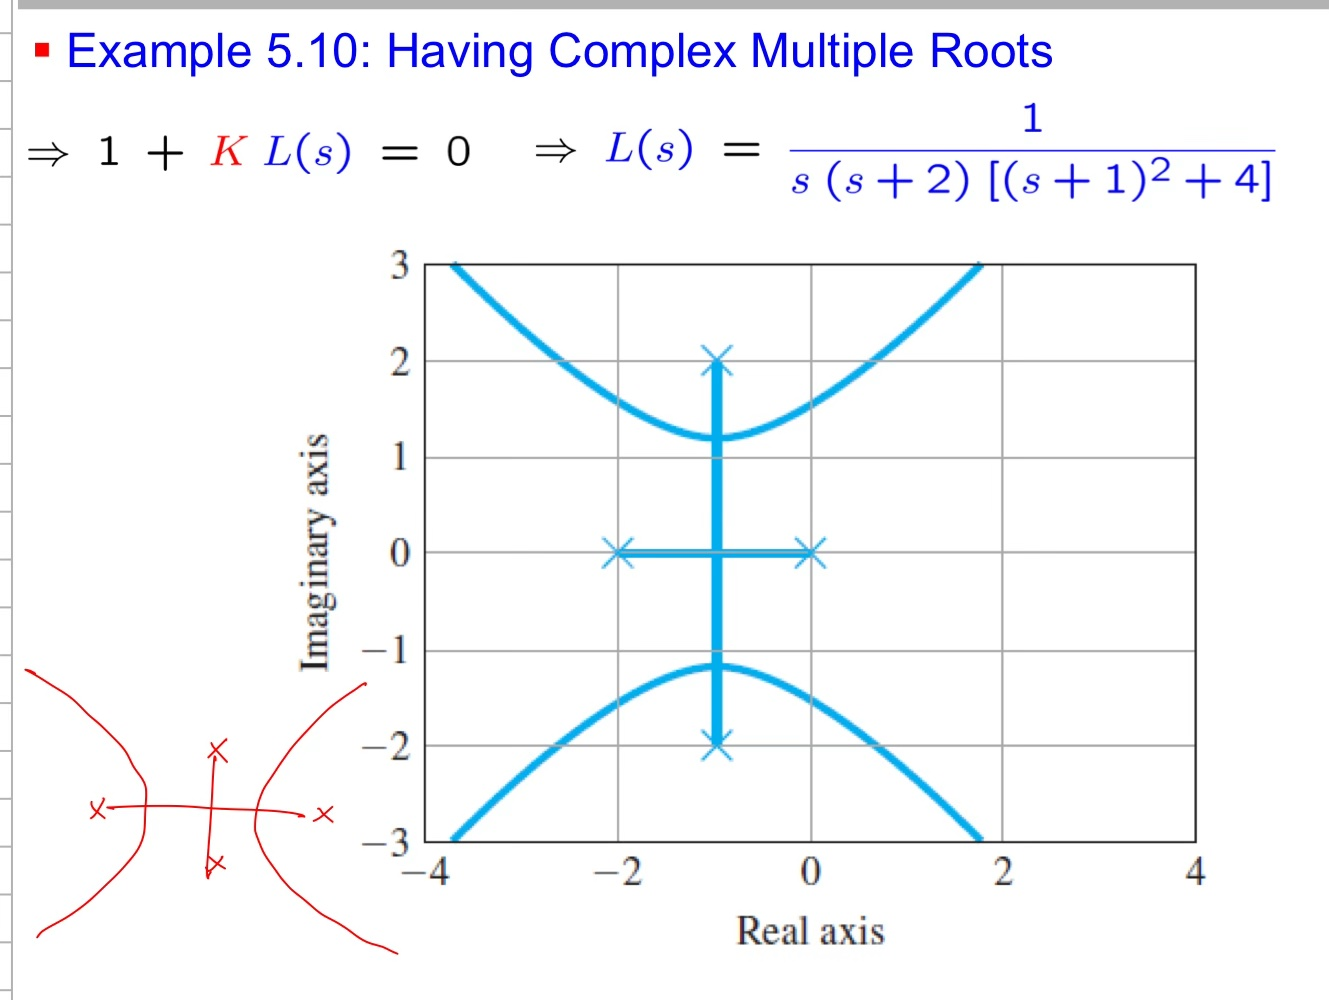
\includegraphics[width=0.55\linewidth]{figs/sketch.jpg}\\[0.2em]
{\small\sffamily 圖 1\quad 講義例 5.10 的根軌跡（藍）與教授上課提出的「）（」形（紅，左下角）}
\end{center}

%==========================================
\section{五條規則分不出兩種形狀}
把例 5.10 推廣成
\[
L(s)=\frac{1}{s(s+2)[(s+1)^2+\omega^2]},\qquad \omega>0,
\]
講義的例子是 $\omega=2$。依講義的五條規則逐一檢查：

\begin{tabularx}{\linewidth}{>{\raggedright}p{1.6cm}X}
\toprule
規則 & 結果\tabularnewline\midrule
Rule 1 & 4 條分支從 $0,-2,-1\pm j\omega$ 出發，沒有零點，全部走向 $\infty$。\tabularnewline
Rule 2 & 實軸段為 $-2\le s\le0$。\tabularnewline
Rule 3 & $\alpha=\dfrac{0-2-1-1}{4}=-1$，角度 $\pm45^\circ,\pm135^\circ$。\tabularnewline
Rule 4 & 從 $-1+j\omega$ 出發：$\phi=-\left[(180^\circ-\tan^{-1}\omega)+\tan^{-1}\omega+90^\circ\right]+180^\circ=-90^\circ$。\tabularnewline
Rule 5 & 重根的位置與 $\omega$ 有關（見第 3 節）。\tabularnewline
\bottomrule
\end{tabularx}

Rule 1--4 的結果\textbf{完全不含 $\omega$}：不論複數極點高低，實軸段、漸近線、出發角（垂直向下）都一樣。兩種形狀都滿足這四條規則，差別只在分支「在哪裡、以什麼順序」相遇，所以要靠重根的計算來決定。

%==========================================
\section{利用對稱性直接解出根的走向}
\begin{derivationbox}[完整推導：以 $w=s+1$ 代換]
\begin{enumerate}[leftmargin=2.2em]
  \item \textbf{代換}：所有極點對稱於 $s=-1$，令 $s=-1+w$：
  \[
  s(s+2)=(w-1)(w+1)=w^2-1,\qquad (s+1)^2+\omega^2=w^2+\omega^2 .
  \]
  \item \textbf{特徵方程式變成 $w^2$ 的二次式}：
  \begin{align*}
  (w^2-1)(w^2+\omega^2)+K=0
  \;\Rightarrow\;
  w^4+(\omega^2-1)w^2+(K-\omega^2)=0 .
  \end{align*}
  \item \textbf{解 $w^2$}：
  \[
  \boxed{\,w^2=\frac{(1-\omega^2)\pm\sqrt{(1+\omega^2)^2-4K}}{2}\,}
  \]
  $w^2>0$ 表示根在實軸上（$s=-1\pm\sqrt{w^2}$）；$w^2<0$ 表示根在直線 $\operatorname{Re}s=-1$ 上（$s=-1\pm j\sqrt{-w^2}$）；$w^2$ 為複數表示根已離開這兩條線。
  \item \textbf{第一次相遇}：兩個 $w^2$ 的乘積為 $K-\omega^2$，所以 $K_1=\omega^2$ 時其中一個 $w^2=0$，兩個根在 $s=-1$ 會合；另一個 $w^2=1-\omega^2$。
  \item \textbf{第二次相遇}：判別式為零時兩個 $w^2$ 相等：
  \[
  K^*=\frac{(1+\omega^2)^2}{4},\qquad w^{*2}=\frac{1-\omega^2}{2}.
  \]
  $K>K^*$ 後 $w^2$ 變成複數，四個根離開對稱線，走向 $\pm45^\circ,\pm135^\circ$ 漸近線。
\end{enumerate}
\end{derivationbox}

關鍵在於 $1-\omega^2$ 的正負號，它決定 $K_1$ 時\textbf{誰}在 $-1$ 會合，以及 $K^*$ 時重根在實軸上還是在虛數處。

%==========================================
\section{三種情況}

\begin{tabularx}{\linewidth}{>{\raggedright}p{2.2cm}>{\raggedright}p{4.6cm}X}
\toprule
情況 & $K_1=\omega^2$（在 $-1$ 會合） & $K^*=\frac{(1+\omega^2)^2}{4}$（第二次相遇）\tabularnewline\midrule
$\omega>1$ & \textbf{實軸分支}（來自 $0$、$-2$）會合，之後沿 $\operatorname{Re}s=-1$ 上下分開 & $w^{*2}<0$：在 $s=-1\pm j\sqrt{\frac{\omega^2-1}{2}}$ 形成\textbf{複數重根}\tabularnewline
$\omega=1$ & $K_1=K^*=1$ & 四個根同時在 $s=-1$ 重合（四重根），以 $45^\circ$ 方向、間隔 $90^\circ$ 離開\tabularnewline
$\omega<1$ & \textbf{複數極點}垂直往下會合，之後沿實軸左右分開 & $w^{*2}>0$：在 $s=-1\pm\sqrt{\frac{1-\omega^2}{2}}$ 形成\textbf{實軸分離點}，垂直離開後彎向漸近線，即「）（」形\tabularnewline
\bottomrule
\end{tabularx}

\textbf{數值驗算}（Python）：
\begin{itemize}[leftmargin=1.5em]
  \item $\omega=2$（講義）：$K_1=4$ 在 $-1$ 會合；$K^*=6.25$，複數重根 $-1\pm1.22j$，與講義圖一致。
  \item $\omega=1$：$K=1$ 時四個根都在 $-1$。
  \item $\omega=0.5$：$K_1=0.25$ 複數極點在 $-1$ 會合；$K^*=0.39$，分離點 $s=-0.39$、$-1.61$。
\end{itemize}

\begin{center}
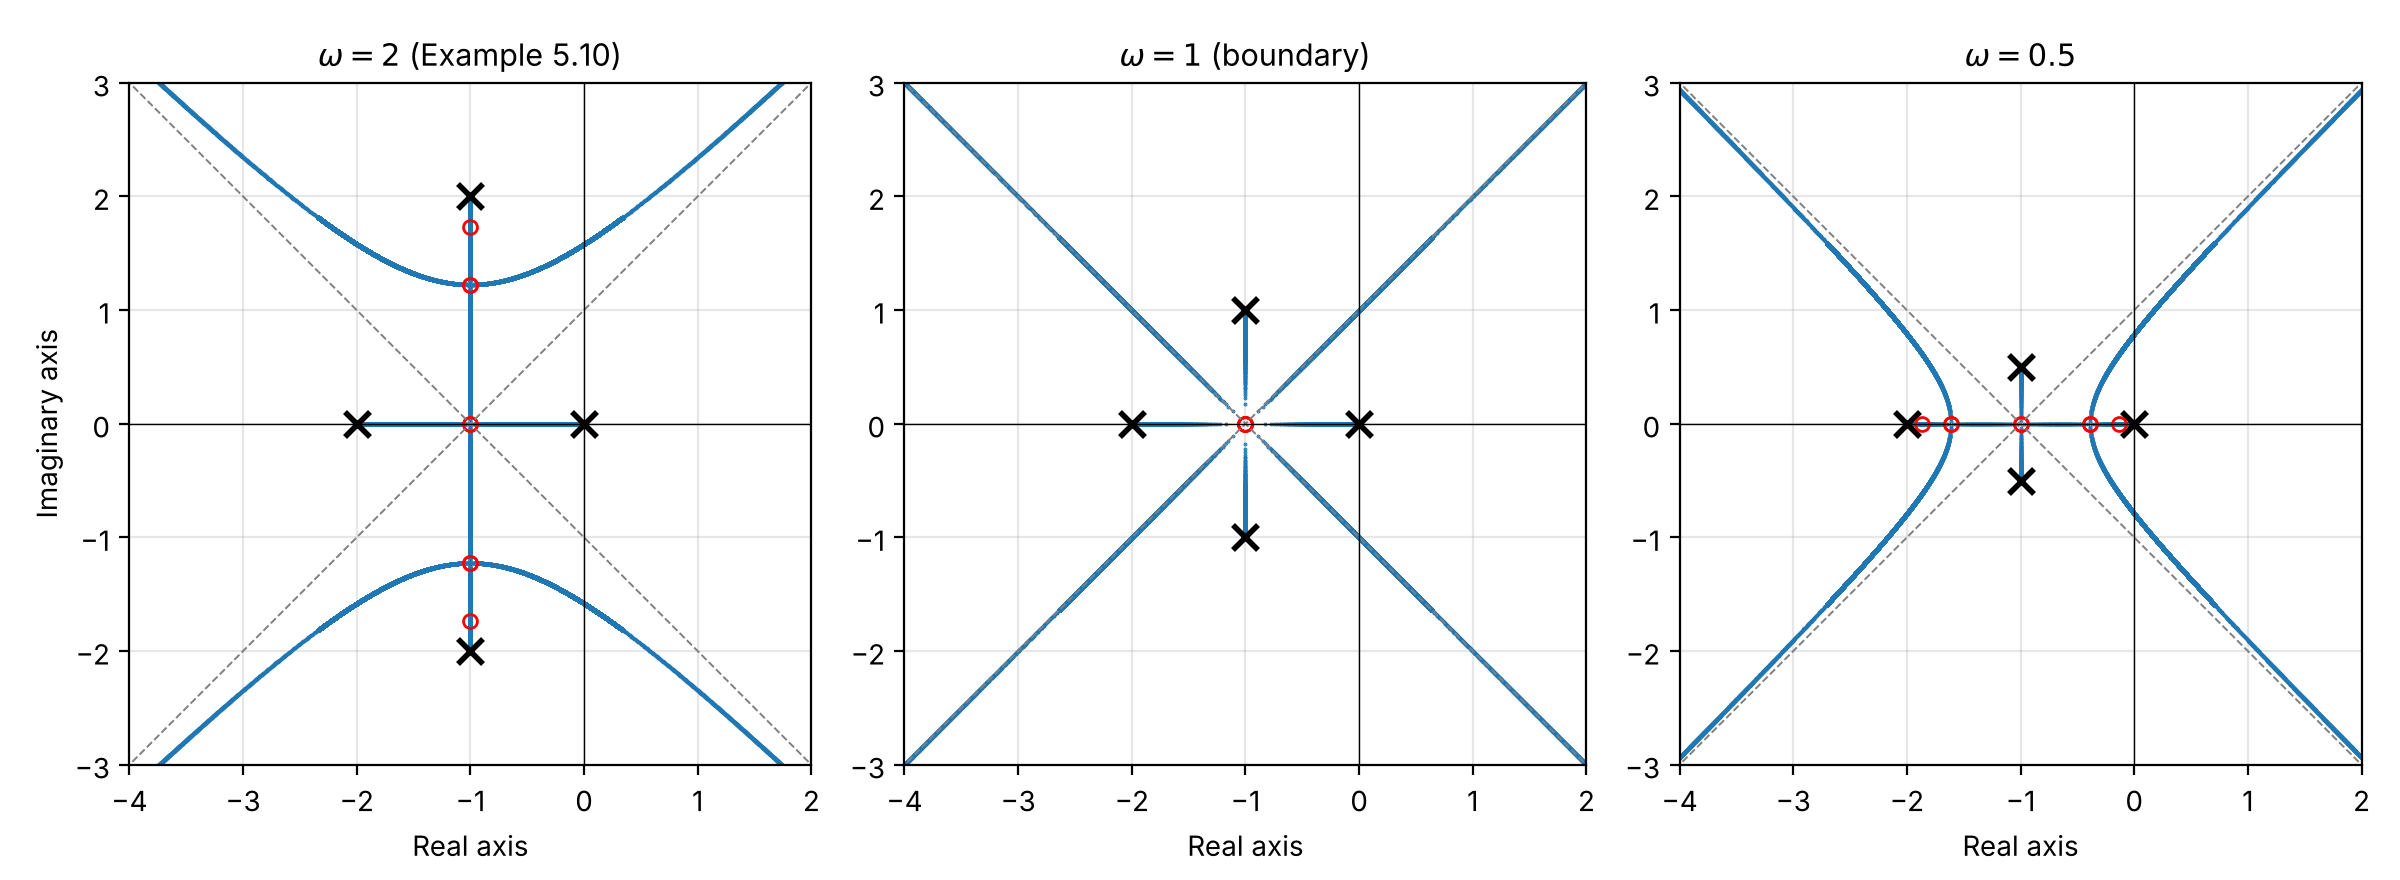
\includegraphics[width=\linewidth]{figs/three_cases.png}\\[0.2em]
{\small\sffamily 圖 2\quad 三種 $\omega$ 的根軌跡（×為開迴路極點，紅圈為 $K_1$、$K^*$ 時的根，虛線為漸近線）}
\end{center}

圖 3 畫出兩個 $w^2$ 隨 $K$ 的變化。$\omega=2$ 時，藍線先穿過 $0$（實軸分支在 $-1$ 會合），兩條線再在負值處合併（複數重根）；$\omega=0.5$ 時，橘線先穿過 $0$（複數極點在 $-1$ 會合），兩條線在正值處合併（實軸分離點）。

\begin{center}
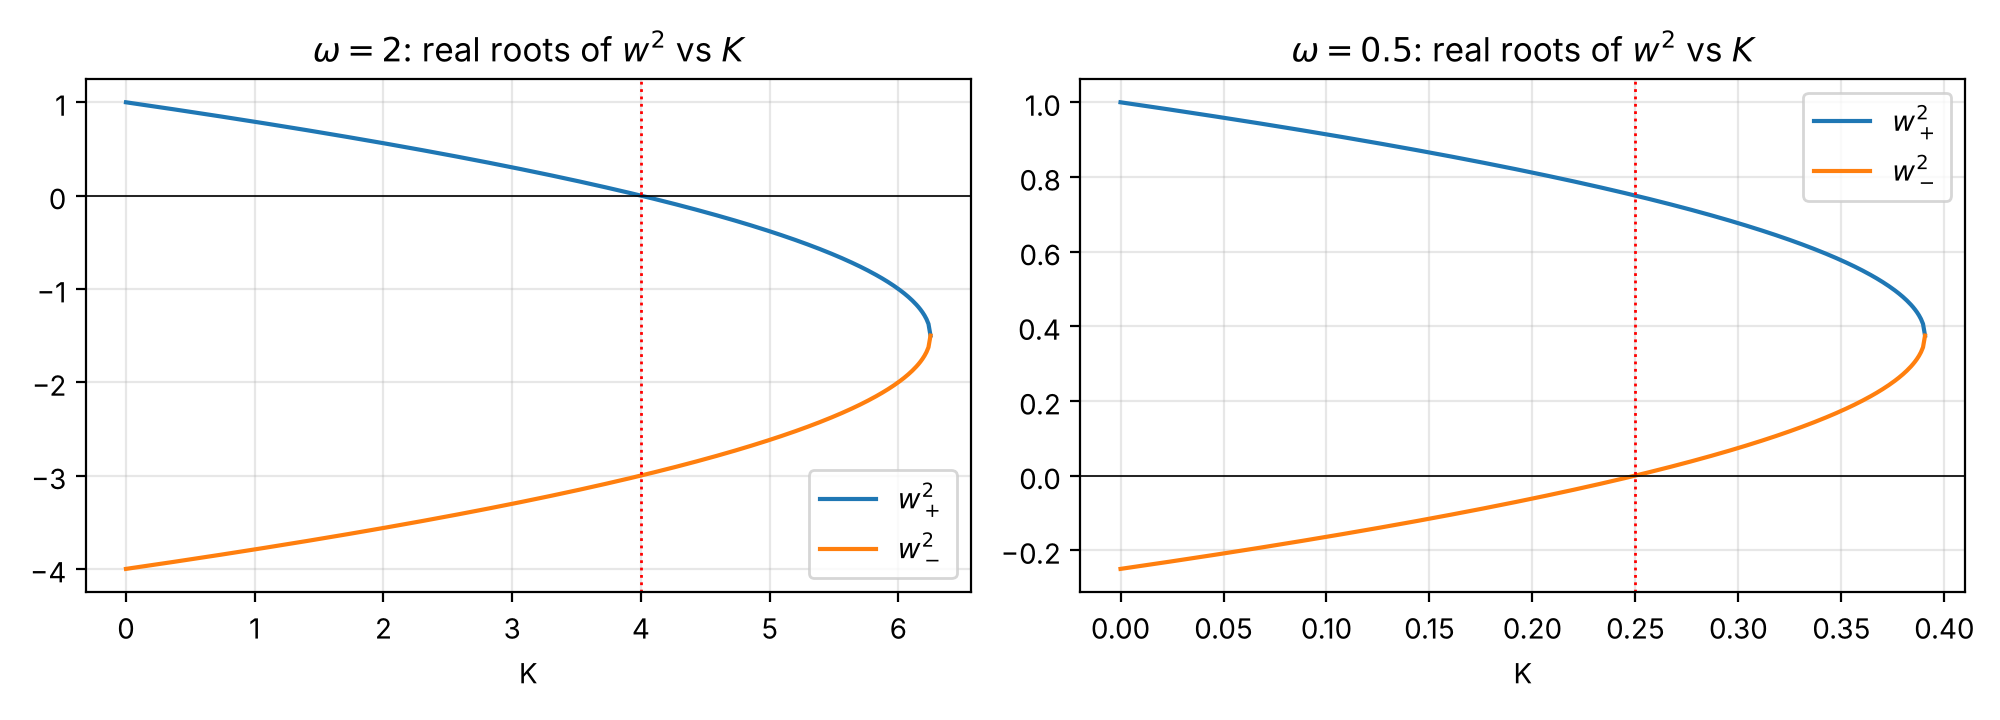
\includegraphics[width=0.92\linewidth]{figs/w2_vs_K.png}\\[0.2em]
{\small\sffamily 圖 3\quad 兩個 $w^2$ 隨 $K$ 的變化（紅色虛線為 $K_1=\omega^2$）}
\end{center}

%==========================================
\section{手繪時的判斷準則}
把實數極點放在 $0$、$-2a$，複數極點放在 $-a\pm j\omega$，同樣令 $s=-a+w$：
\[
(w^2-a^2)(w^2+\omega^2)+K=0\;\Rightarrow\;w^2=\frac{(a^2-\omega^2)\pm\sqrt{(a^2+\omega^2)^2-4K}}{2}.
\]
所以準則是比較\textbf{複數極點的虛部 $\omega$} 與\textbf{兩實數極點間距的一半 $a$}：
\begin{itemize}[leftmargin=1.5em]
  \item $\omega>a$：講義例 5.10 的形狀（複數重根）。
  \item $\omega=a$：四重根，四條分支沿漸近線直接離開。
  \item $\omega<a$：「）（」形（實軸上兩個分離點）。
\end{itemize}

\textbf{檢查手繪圖的要點}：「）（」的兩條曲線必須在 $[-2a,0]$ 之間穿過實軸（分離點 $-a\pm\sqrt{(a^2-\omega^2)/2}$ 一定落在這個區間內）。若畫成在 $-2a$ 左邊或 $0$ 右邊穿過實軸就是錯的，因為那些點右邊的實數極點數為偶數，依 Rule 2 不在軌跡上。

%==========================================
\section{結論與學習回授}
\begin{recipebox}[結論]
\begin{enumerate}
  \item 教授提出的「）（」形確實可能出現，只是要在 $\omega<1$ 的參數範圍，不是例 5.10 本身（$\omega=2$）。
  \item 對這類「兩實極點＋一對複數極點、且對稱」的系統，Rule 1--4 無法區分形狀；要用對稱代換 $s=-a+w$ 解出重根位置，或比較 $\omega$ 與 $a$。
\end{enumerate}
\end{recipebox}

\textbf{學習回授}：
\begin{itemize}[leftmargin=1.5em]
  \item \textbf{我的收穫}：之前以為五條規則套完就能畫出唯一的形狀。這次發現規則只給「骨架」，分支在哪裡相遇要另外算；對稱的系統可以用代換把四次方程式降成二次，這個技巧很好用。
  \item \textbf{仍想確認的問題}：考試手繪這類題目時，是否要求寫出複數重根的位置與對應 $K$，還是只要畫出正確的形狀即可？
\end{itemize}

\end{document}
